%package list
\documentclass{article}
\usepackage[top=3cm, bottom=3cm, outer=3cm, inner=3cm]{geometry}
\usepackage{multicol}
\usepackage{graphicx}
\usepackage{url}
%\usepackage{cite}
\usepackage{hyperref}
\usepackage{array}
%\usepackage{multicol}
\newcolumntype{x}[1]{>{\centering\arraybackslash\hspace{0pt}}p{#1}}
\usepackage{natbib}
\usepackage{pdfpages}
\usepackage{multirow}
\usepackage[normalem]{ulem}
\useunder{\uline}{\ul}{}
\usepackage{svg}
\usepackage{xcolor}
\usepackage{listings}
\lstdefinestyle{ascii-tree}{
    literate={├}{|}1 {─}{--}1 {└}{+}1 
  }
\lstset{basicstyle=\ttfamily,
  showstringspaces=false,
  commentstyle=\color{red},
  keywordstyle=\color{blue}
}
%\usepackage{booktabs}
\usepackage{caption}
\usepackage{subcaption}
\usepackage{float}
\usepackage{array}

\newcolumntype{M}[1]{>{\centering\arraybackslash}m{#1}}
\newcolumntype{N}{@{}m{0pt}@{}}


%%%%%%%%%%%%%%%%%%%%%%%%%%%%%%%%%%%%%%%%%%%%%%%%%%%%%%%%%%%%%%%%%%%%%%%%%%%%
%%%%%%%%%%%%%%%%%%%%%%%%%%%%%%%%%%%%%%%%%%%%%%%%%%%%%%%%%%%%%%%%%%%%%%%%%%%%
\newcommand{\itemEmail}{rcompanocca@unsa.edu.pe}
\newcommand{\itemStudent}{Roni Companocca Checco}
\newcommand{\itemCourse}{Programación}
\newcommand{\itemCourseCode}{20210558}
\newcommand{\itemSemester}{II}
\newcommand{\itemUniversity}{Universidad Nacional de San Agustín de Arequipa}
\newcommand{\itemFaculty}{Facultad de Ingeniería de Producción y Servicios}
\newcommand{\itemDepartment}{Departamento Académico de Ingeniería de Sistemas e Informática}
\newcommand{\itemSchool}{Escuela Profesional de Ingeniería de Sistemas}
\newcommand{\itemAcademic}{2023 - B}
\newcommand{\itemInput}{Del 14 Diciembre 2023}
\newcommand{\itemOutput}{Al 20 Diciembre 2023}
\newcommand{\itemPracticeNumber}{22}
\newcommand{\itemTheme}{ Interfaz Gráfica de Usuario }
%%%%%%%%%%%%%%%%%%%%%%%%%%%%%%%%%%%%%%%%%%%%%%%%%%%%%%%%%%%%%%%%%%%%%%%%%%%%
%%%%%%%%%%%%%%%%%%%%%%%%%%%%%%%%%%%%%%%%%%%%%%%%%%%%%%%%%%%%%%%%%%%%%%%%%%%%

\usepackage[english,spanish]{babel}
\usepackage[utf8]{inputenc}
\AtBeginDocument{\selectlanguage{spanish}}
\renewcommand{\figurename}{Figura}
\renewcommand{\refname}{Referencias}
\renewcommand{\tablename}{Tabla} %esto no funciona cuando se usa babel
\AtBeginDocument{%
	\renewcommand\tablename{Tabla}
}

\usepackage{fancyhdr}
\pagestyle{fancy}
\fancyhf{}
\setlength{\headheight}{30pt}
\renewcommand{\headrulewidth}{1pt}
\renewcommand{\footrulewidth}{1pt}
\fancyhead[L]{\raisebox{-0.2\height}{
\includegraphics[width=3cm]{logo_episunsa.png}}}
\fancyhead[C]{\fontsize{7}{7}\selectfont	\itemUniversity \\ \itemFaculty \\ \itemDepartment \\ \itemSchool \\ \textbf{\itemCourse}}
\fancyhead[R]{\raisebox{-0.2\height}{
\includegraphics[width=1.2cm]{abet.png}}}
\fancyfoot[L]{Estudiante Roni Companocca Checco}
\fancyfoot[C]{\itemCourse}
\fancyfoot[R]{Página \thepage}

% para el codigo fuente
\usepackage{listings}
\usepackage{color, colortbl}
\definecolor{dkgreen}{rgb}{0,0.6,0}
\definecolor{gray}{rgb}{0.5,0.5,0.5}
\definecolor{mauve}{rgb}{0.58,0,0.82}
\definecolor{codebackground}{rgb}{0.95, 0.95, 0.92}
\definecolor{tablebackground}{rgb}{0.8, 0, 0}

\lstset{frame=tb,
	language=bash,
	aboveskip=3mm,
	belowskip=3mm,
	showstringspaces=false,
	columns=flexible,
	basicstyle={\small\ttfamily},
	numbers=none,
	numberstyle=\tiny\color{gray},
	keywordstyle=\color{blue},
	commentstyle=\color{dkgreen},
	stringstyle=\color{mauve},
	breaklines=true,
	breakatwhitespace=true,
	tabsize=3,
	backgroundcolor= \color{codebackground},
}

\begin{document}
	
	\vspace*{10px}
	
	\begin{center}	
		\fontsize{17}{17} \textbf{ Informe de Laboratorio \itemPracticeNumber}
	\end{center}
	\centerline{\textbf{\Large Tema: \itemTheme}}
	%\vspace*{0.5cm}	

	\begin{flushright}
		\begin{tabular}{|M{2.5cm}|N|}
			\hline 
			\rowcolor{tablebackground}
			\color{white} \textbf{Nota}  \\
			\hline 
			     \\[30pt]
			\hline 			
		\end{tabular}
	\end{flushright}	

	\begin{table}[H]
		\begin{tabular}{|x{4.7cm}|x{4.8cm}|x{4.8cm}|}
			\hline 
			\rowcolor{tablebackground}
			\color{white} \textbf{Estudiante} & \color{white}\textbf{Escuela}  & \color{white}\textbf{Asignatura}   \\
			\hline 
			{\itemStudent \par \itemEmail} & \itemSchool & {\itemCourse \par Semestre: \itemSemester \par Código: \itemCourseCode}     \\
			\hline 			
		\end{tabular}
	\end{table}		
	
	\begin{table}[H]
		\begin{tabular}{|x{4.7cm}|x{4.8cm}|x{4.8cm}|}
			\hline 
			\rowcolor{tablebackground}
			\color{white}\textbf{Laboratorio} & \color{white}\textbf{Tema}  & \color{white}\textbf{Duración}   \\
			\hline 
			\itemPracticeNumber & \itemTheme & 04 horas   \\
			\hline 
		\end{tabular}
	\end{table}
	
	\begin{table}[H]
		\begin{tabular}{|x{4.7cm}|x{4.8cm}|x{4.8cm}|}
			\hline 
			\rowcolor{tablebackground}
			\color{white}\textbf{Semestre académico} & \color{white}\textbf{Fecha de inicio}  & \color{white}\textbf{Fecha de entrega}   \\
			\hline 
			\itemAcademic & \itemInput &  \itemOutput  \\
			\hline 
		\end{tabular}
	\end{table}

    \section{TAREA}
	\begin{itemize}	
    \subsection{Objetivos:}
		\item Crear componentes gráficos básicos
		\item Utilizar la interfaz ActionListener 
        \item Crear inner classes 
       
    \subsection{Competencias a alcanzar:}
		\item Diseña, responsablemente, sistemas, componentes o procesos para satisfacer necesidades dentro de restricciones realistas: económicas, medio ambientales, sociales, políticas, éticas, de salud, de seguridad, manufacturación y sostenibilidad. 
        \item Aplica de forma flexible, técnicas, métodos, principios, normas, estándares y herramientas de ingeniería necesarias para la construcción de software e implementación de sistemas de información.
    \end{itemize}

    \section{EQUIPOS, MATERIALES Y TEMAS UTILIZADOS}
	\begin{itemize}
		\item Sistema Operativo Windows
		\item OpenJDK 64-Bits 17.0.7.
		\item Git 2.39.2.	
  	\item Cuenta en GitHub con el correo institucional.
	\end{itemize}

    \section{URL DE REPOSITORIO GITHUB}
	\begin{itemize}
		\item URL para el Repositorio GitHub.
		\item \url{https://github.com/RONI-COMPANOCCA-CHECCO}
		\item URL para el laboratorio 22 en el Repositorio GitHub.	
        \item \url{https://github.com/RONI-COMPANOCCA-CHECCO/FP2-LAB22}
	\end{itemize}
    
    \section{CODIGO DEL VIDEOJUEGO DE ESTRATEGIA Y SU DIAGRAMA UML}
	\begin{itemize}

        \item clase Arquero.java
        \begin{lstlisting}[language=java]
public class Arquero extends Soldado {
    private int numeroFlechas;
    private static int num = 0;

    public Arquero(String s, int ata, int def, int vid, int cant){
        super(s,ata,def,vid);
        numeroFlechas = cant;
        num++;
    }

    public void disparar(){
        if(numeroFlechas>0){
            numeroFlechas--;
        }
    }

    public static int cuantos(){
        return num;
    }

    public static void resetearCantidad(){
        num = 0;
    }
    
    public String toString(){
        return super.toString()+" "+numeroFlechas;
    }
}
        \end{lstlisting}

        \item clase Caballero.java
        \begin{lstlisting}[language=java]
public class Caballero extends Soldado{
    private String armaActual = "lanza";
    private boolean montando = true;
    private static int num = 0;

    public Caballero(String s, int ata, int def, int vid){
        super(s,ata,def,vid);
        num++;
    }

    public void envestir(){
        if(montando==true){
            for(int i=0; i<=2; i++){
                super.atacar();
            }
        }else{
            super.atacar();
        }
    }

    public void desmontar(){
        if(montando==true){
            montando = false;
            super.defender();
            cambiaArma();
        }
    }

    public void cambiaArma(){
        if(armaActual=="lanza"){
            armaActual = "Espada";
        }else{
            armaActual = "lanza";
        }
    }

    public void montar(){
        if(montando==false){
            montando = true;
            super.atacar();
            cambiaArma();
        }
    }
    
    public static int cuantos(){
        return num;
    }

    public static void resetearCantidad(){
        num=0;
    }

    public String toString(){
        return super.toString()+" "+armaActual+" "+montando;
    }
}

        \end{lstlisting}

        \item clase Espadachin.java
        \begin{lstlisting}[language=java]
public class Espadachin extends Soldado{
    private int longitudEspada;
    private boolean muroEscudos = false;
    private static int num = 0;

    public Espadachin(String s, int ata, int def, int vid, int lon){
        super(s,ata,def,vid);
        longitudEspada = lon;
        num++;
    }

    public void muroEscudos(){
        if(muroEscudos == true ){
            muroEscudos = false;
        }else{
            muroEscudos = true;
        }
    }

    public static int cuantos(){
        return num;
    }

    public static void resetearCantidad(){
        num =0;
    }

    public String toString(){
        return super.toString()+" "+longitudEspada+" "+muroEscudos;
    }
}
        \end{lstlisting}

        \item clase Lancero.java
        \begin{lstlisting}[language=java]
public class Lancero extends Soldado {
    private int longitudLanza;
    private static int num = 0;

    public Lancero(String nombre, int ataque, int defensa, int vida, int longitudLanza) {
        super(nombre, ataque, defensa, vida);
        this.longitudLanza = longitudLanza;
        num++;
    }

    // Método específico para la acción "schiltrom"
    public void schiltrom() {
        if (getActitud().equals("defensa")) {
            // Aumentar el nivel de defensa en 1 cuando se realiza schiltrom
            setNivelDefensa(getNivelDefensa() + 1);
        }
    }

    // Sobrescribe el método serAtacado para personalizar la acción en caso de ataque
    @Override
    public void serAtacado() {
        // Realiza schiltrom antes de recibir el ataque
        schiltrom();
        // Llama al método de la superclase para aplicar el daño
        super.serAtacado();
    }

    public static int cuantos(){
        return num;
    }

    public static void resetearCantidad(){
        num =0;
    }

    // Sobrescribe el método toString para agregar información específica de Lancero
    @Override
    public String toString() {
        return super.toString() + " Longitud de lanza: " + longitudLanza;
    }
}
        \end{lstlisting}

        \item clase Ejercito.java
        \begin{lstlisting}[language=java]
import java.util.*;
public class Ejercito {
    ArrayList<Soldado> misSoldados = new ArrayList<Soldado>();
    String cultura;

    public Ejercito(String cult, int cantidad){
        cultura = cult;
        int tipo;
        for(int i=0; i<cantidad; i++){
            tipo = (int)(Math.random()*4)+1;
            switch (tipo) {
                case 1: misSoldados.add(new Espadachin("\nE: "+i, 10, 8, 10, 40));
                    break;
            
                case 2: misSoldados.add(new Caballero("\nC: "+i, 13, 7, 12));
                    break;

                case 3: misSoldados.add(new Arquero("\nA: "+i, 7, 3, 5, 20));
                    break;

                case 4: misSoldados.add(new Lancero("\nL: "+i, 5, 10, 8, 20));
                    break;
            }
        }
    }

    public String toString(){
        String todos ="";
        for(int i=0; i<misSoldados.size(); i++){
            todos += misSoldados.get(i)+"";
        }
        return cultura+" "+misSoldados.size()+" "+todos;
    }

    public int poder(){
        int poder = 0;
        for(int i=0; i<misSoldados.size(); i++){
            poder += misSoldados.get(i).getVida();
        }
        return poder;
    }

    public String getCultura(){
        return cultura;
    }

    public static void resetearCantidad(){
        Soldado.resetearCantidad();
        Arquero.resetearCantidad();
        Caballero.resetearCantidad();
        Espadachin.resetearCantidad();
        Lancero.resetearCantidad();
    }
}
        \end{lstlisting}

        \item clase Mapa.java
        \begin{lstlisting}[language=java]
import java.util.Random;

public class Mapa {
    private String tipoTerritorio;
    private Soldado[][] tablero;

    // Constructor
    public Mapa(String tipoTerritorio) {
        this.tipoTerritorio = tipoTerritorio;
        this.tablero = new Soldado[10][10]; // Tamaño del tablero (puedes ajustarlo según tus necesidades)
        posicionarSoldadosAleatorios();
    }

    // Método para posicionar soldados aleatorios en el tablero
    private void posicionarSoldadosAleatorios() {
        Random rand = new Random();
        for (int i = 0; i < 10; i++) { // Número arbitrario de soldados por ejército
            int fila = rand.nextInt(10);
            int columna = rand.nextInt(10);

            // Verificar si la posición está ocupada
            while (tablero[fila][columna] != null) {
                fila = rand.nextInt(10);
                columna = rand.nextInt(10);
            }

            // Crear un soldado aleatorio (puedes ajustar estos valores según tus necesidades)
            Soldado soldado = new Soldado("Soldado" + i, 8, 5, rand.nextInt(5) + 5);
            tablero[fila][columna] = soldado;
        }
    }

    // Método para mostrar el tablero
    public void mostrarTablero() {
        System.out.println("Mapa - Tipo de Territorio: " + tipoTerritorio);
        for (Soldado[] fila : tablero) {
            for (Soldado soldado : fila) {
                if (soldado != null) {
                    System.out.print(soldado.getNombre() + " ");
                } else {
                    System.out.print("Vacío ");
                }
            }
            System.out.println();
        }
    }
}
        \end{lstlisting}

        \item clase Soldado.java
        \begin{lstlisting}[language=java]
public class Soldado {
	private String nombre;
    private int nivelAtaque;
    private int nivelDefensa;
    private int nivelVida;
    private int vidaActual;
    private int velocidad = 0;
    private String actitud = "defensa";
    private boolean vive = true;
    private static int num = 0;
	
    //COMSTRUCTORES
	public Soldado(String nomb, int ataque, int defensa, int vida) {
		nombre = nomb;
        nivelAtaque = ataque;
        nivelDefensa = defensa;
        nivelVida = vida;
        vidaActual = vida;
        num++;
	}

	// Otros métodos
    public void atacar() {
        actitud = "ataque";
        avanzar();
    }

    public void defender() {
        actitud = "defensa";
        velocidad = 0;
    }

    public void avanzar() {
        velocidad++;
    }

    public void retroceder() {
        velocidad--;
    }

    public void serAtacado() {
        vidaActual--;
        if (vidaActual == 0) 
            morir();
    }

    public void huir(){
        actitud = "fuga";
        velocidad++;
    }

    public void morir() {
        vive = false;
    }

    public String toString() {
        return nombre+ " " +nivelAtaque+ " "+nivelDefensa+ " " +nivelVida+ " " +vidaActual+ " " +velocidad+ " " +actitud+ " " +vive;
    }

    public static int cuantos(){
        return num;
    }

    public static void resetearCantidad(){
        num=0;
    }

    public int getVida(){
        return nivelVida;
    }

    public String getActitud(){
        return actitud;
    }

    public void setNivelDefensa(int nivelDefensa) {
        this.nivelDefensa = nivelDefensa;
    }

    public int getNivelDefensa(){
        return nivelDefensa;
    }
}
        \end{lstlisting}

        \item clase Main.java
        \begin{lstlisting}[language=java]
// RONI COMPANOCCA CHECCO
// CUI: 20210558
// LABORATORIO 22
// FUNDAMENTOS DE PROGRAMACION 
public class Main {
    public static void main(String[] args){
        int cant;
        String cultura[] = {"Inglaterra","Francia","Sacro Imperio Romano Germanico","Aragon","Moros"};
        cant = aleatorio(1,10);
        Ejercito e1 = new Ejercito(cultura[aleatorio(0,4)], cant);
        mostrar(e1);
        cant = aleatorio(1,10);
        Ejercito e2 = new Ejercito(cultura[aleatorio(0,4)], cant);
        mostrar(e2);
        determinarGanador(e1,e2);
    }
    
    public static int aleatorio(int a, int b){
        return (int)(Math.random()*(b-a+1))+a;
    }

    private static int aux = 1;

    public static void mostrar(Ejercito e){
        System.out.print("Ejercito "+aux+" "+e.getCultura());
        System.out.println("\nCantidad total de Soldados: "+Soldado.cuantos()+"\n"+"Espadachines: "+Espadachin.cuantos()+"\n"+"Arqueros: "+Arquero.cuantos()+"\n"+"Lanceros: "+Lancero.cuantos()+"\n"+"Caballeros: "+Caballero.cuantos()+"\n");
        Ejercito.resetearCantidad();
        aux++;
    }

    public static void determinarGanador(Ejercito e1, Ejercito e2){
        System.out.println("Ejercito 1: "+e1.getCultura()+" con un poder de "+e1.poder());
        System.out.println("Ejercito 2: "+e2.getCultura()+" con un poder de "+e2.poder());
        if (e1.poder()>e2.poder()){
            System.out.println("El ganador es ejercito 1 de : "+e1.getCultura());
        } else if (e1.poder()<e2.poder()){
            System.out.println("El ganador es ejercito 2 de : "+e2.getCultura());
        } else{
            System.out.println("Sin ganador");
        }
    }
}

        \end{lstlisting}
 
             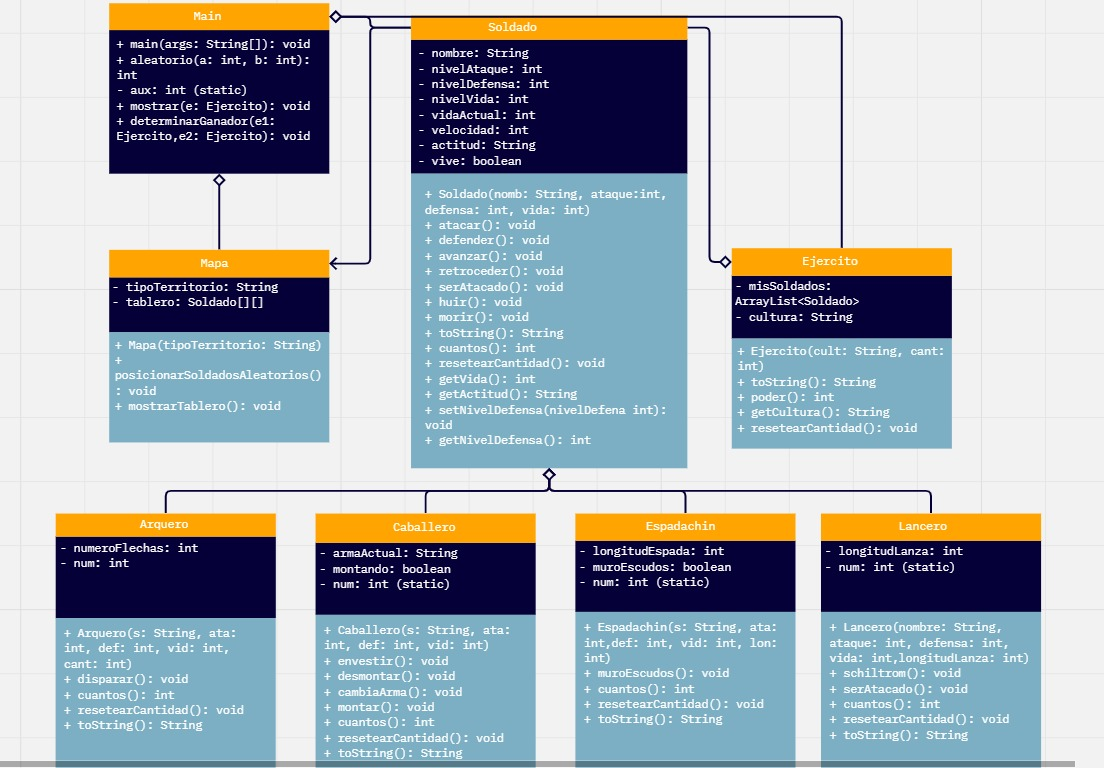
\includegraphics[height=12cm]{uml.jpeg}
        
	\end{itemize}

    \section{ACTIVIDAD}
 \begin{itemize}
		\item Cree una versión del videojuego de estrategia usando componentes básicos GUI: Etiquetas, botones, cuadros de texto, JOptionPane, Color.
		\item Además, utilizar componentes avanzados GUI: Layouts, JPanel, áreas de texto, checkbox, botones de radio y combobox. 
		\item Considerar nivel estratégico y táctico. 
  	\item Considerar hasta las unidades especiales de los reinos.
        \item Hacerlo iterativo. 
        \\
        \begin{lstlisting}[language=java]
import javax.swing.*;
import java.awt.*;
import java.awt.event.ActionEvent;
import java.awt.event.ActionListener;
import java.util.Random;

public class JuegoInterfazAvanzada extends JFrame {

    private JButton botonIniciar;
    private JLabel etiquetaCultura;
    private JComboBox<String> listaCulturas;
    private JCheckBox checkBoxModoEstrategico;
    private JRadioButton radioTactico;
    private JRadioButton radioEstrategico;
    private ButtonGroup grupoRadio;
    private JTextArea areaTexto;
    private JPanel panelJuego;

    public JuegoInterfazAvanzada() {
        super("Juego de Estrategia");

        etiquetaCultura = new JLabel("Seleccione Territorio:");
        listaCulturas = new JComboBox<>(new String[]{"Bosque", "Campo abierto", "Montaña", "Desierto", "Playa"});
        checkBoxModoEstrategico = new JCheckBox("Modo Estratégico");

        radioTactico = new JRadioButton("Táctico");
        radioEstrategico = new JRadioButton("Estratégico");
        grupoRadio = new ButtonGroup();
        grupoRadio.add(radioTactico);
        grupoRadio.add(radioEstrategico);

        areaTexto = new JTextArea(10, 30);
        areaTexto.setEditable(false);
        JScrollPane scrollPane = new JScrollPane(areaTexto);

        botonIniciar = new JButton("Iniciar Juego");
        botonIniciar.addActionListener(new ActionListener() {
            @Override
            public void actionPerformed(ActionEvent e) {
                iniciarJuego();
            }
        });

        panelJuego = new JPanel(new BorderLayout());
        add(panelJuego, BorderLayout.CENTER);

        JPanel panelSuperior = new JPanel(new FlowLayout());
        panelSuperior.add(etiquetaCultura);
        panelSuperior.add(listaCulturas);
        panelSuperior.add(checkBoxModoEstrategico);

        JPanel panelRadio = new JPanel();
        panelRadio.add(radioTactico);
        panelRadio.add(radioEstrategico);

        JPanel panelCentral = new JPanel(new BorderLayout());
        panelCentral.add(panelSuperior, BorderLayout.NORTH);
        panelCentral.add(panelRadio, BorderLayout.CENTER);
        panelCentral.add(scrollPane, BorderLayout.SOUTH);

        JPanel panelBoton = new JPanel();
        panelBoton.add(botonIniciar);

        add(panelCentral, BorderLayout.CENTER);
        add(panelBoton, BorderLayout.SOUTH);

        setDefaultCloseOperation(JFrame.EXIT_ON_CLOSE);
        pack();
        setLocationRelativeTo(null);
        setVisible(true);
    }

    private void iniciarJuego() {
        String selectedCultura = (String) listaCulturas.getSelectedItem();
        boolean modoEstrategico = checkBoxModoEstrategico.isSelected();
        String modoJuego = radioTactico.isSelected() ? "Táctico" : "Estratégico";

        String mensaje = "Iniciando juego con Cultura: " + selectedCultura + "\nModo de Juego: " + modoJuego;
        if (modoEstrategico) {
            mensaje += "\nModo Estratégico Activado";
            ejecutarJuegoEstrategico();
        } else {
            mensaje += "\nModo Táctico Activado";
            JOptionPane.showMessageDialog(this, "Ejecutando lógica del juego táctico...", "Modo Táctico", JOptionPane.INFORMATION_MESSAGE);
            reiniciarJuego();
        }

        areaTexto.setText(mensaje);
    }

    private void ejecutarJuegoEstrategico() {
        // Lógica específica del modo estratégico
        System.out.println("Ejecutando lógica del juego estratégico...");
    }

    private void mostrarResultado(Ejercito e1, Ejercito e2) {
        StringBuilder resultado = new StringBuilder();
        
        // Mostrar detalles del Ejército 1
        resultado.append("Ejercito 1: ").append(e1.getCultura()).append("\n");
        resultado.append("Cantidad total de Soldados: ").append(e1.misSoldados.size()).append("\n");
        resultado.append("Espadachines: ").append(Espadachin.cuantos()).append("\n");
        resultado.append("Arqueros: ").append(Arquero.cuantos()).append("\n");
        resultado.append("Lanceros: ").append(Lancero.cuantos()).append("\n");
        resultado.append("Caballeros: ").append(Caballero.cuantos()).append("\n\n");
    
        // Mostrar detalles del Ejército 2
        resultado.append("Ejercito 2: ").append(e2.getCultura()).append("\n");
        resultado.append("Cantidad total de Soldados: ").append(e2.misSoldados.size()).append("\n");
        resultado.append("Espadachines: ").append(Espadachin.cuantos()).append("\n");
        resultado.append("Arqueros: ").append(Arquero.cuantos()).append("\n");
        resultado.append("Lanceros: ").append(Lancero.cuantos()).append("\n");
        resultado.append("Caballeros: ").append(Caballero.cuantos()).append("\n\n");
    
        // Mostrar el nivel de poder de cada ejército
        resultado.append("Nivel de poder Ejercito 1: ").append(e1.poder()).append("\n");
        resultado.append("Nivel de poder Ejercito 2: ").append(e2.poder()).append("\n\n");

        // Mostrar el resumen del poder de ambos ejércitos
        resultado.append("El ganador es: ");
        if (e1.poder() > e2.poder()) {
            resultado.append("Ejercito 1 de : ").append(e1.getCultura());
        } else if (e1.poder() < e2.poder()) {
            resultado.append("Ejercito 2 de : ").append(e2.getCultura());
        } else {
            resultado.append("Sin ganador");
        }
    
        areaTexto.setText(resultado.toString());
    }

    private Ejercito generarEjercitoAleatorio() {
    // Generar una cultura aleatoria
    String[] culturas = {"Inglaterra", "Francia", "Sacro Imperio Romano Germanico", "Aragon", "Moros"};
    String culturaAleatoria = culturas[new Random().nextInt(culturas.length)];

    // Generar una cantidad aleatoria de soldados (entre 1 y 10)
    int cantidadSoldados = new Random().nextInt(10) + 1;

    // Crear un ejército con soldados aleatorios
    return new Ejercito(culturaAleatoria, cantidadSoldados);
    }

    private void reiniciarJuego() {
        // Volver a ejecutar la lógica del juego y actualizar el contenido en el panel
        SwingUtilities.invokeLater(new Runnable() {
            @Override
            public void run() {
                panelJuego.removeAll(); // Limpiar el panel actual

                // Generar ejércitos aleatorios
                Ejercito e1 = generarEjercitoAleatorio();
                Ejercito e2 = generarEjercitoAleatorio();

                // Mostrar el resultado del juego en el panel
                mostrarResultado(e1, e2);
                revalidate(); // Actualizar la interfaz
                repaint();    // Repintar la interfaz
            }
        });
    }

    public static void main(String[] args) {
        SwingUtilities.invokeLater(new Runnable() {
            @Override
            public void run() {
                new JuegoInterfazAvanzada();
            }
        });
    }

}

        \end{lstlisting}
        \centering
        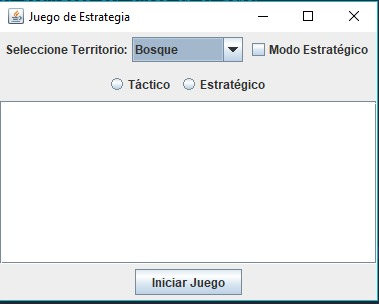
\includegraphics[height=8cm]{im1.jpeg}
        \\
        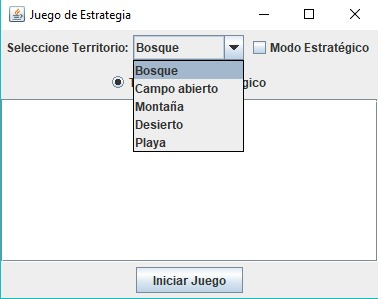
\includegraphics[height=8cm]{im2.jpeg}
        \\
        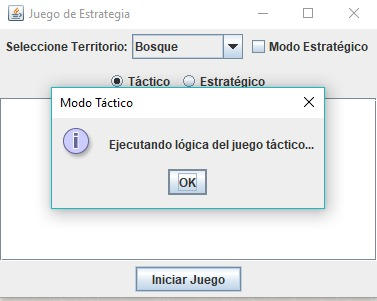
\includegraphics[height=8cm]{im3.jpeg}
        \\
        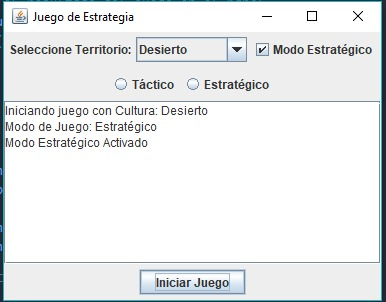
\includegraphics[height=8cm]{im4.jpeg}
        \\
        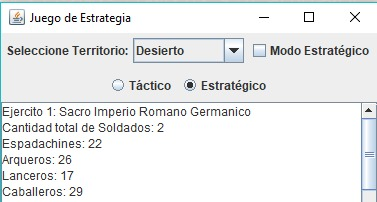
\includegraphics[height=6cm]{im5.jpeg}
        \\
        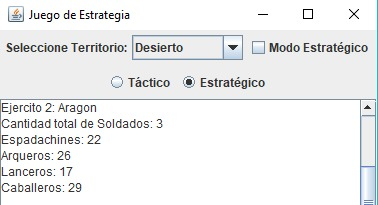
\includegraphics[height=6cm]{im6.jpeg}
        \\
        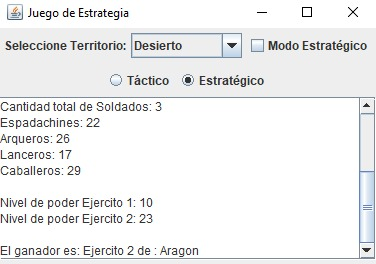
\includegraphics[height=8cm]{im7.jpeg}
        \\
	\end{itemize}

	\section{REFERENCIAS}
	\begin{itemize}
		\item M. Aedo, “Fundamentos de Programación 2 - Tópicos de Programación Orientada a Objetos”, Primera Edición, 2021, Editorial UNSA.
		\item \url{https://github.com/rescobedoq/programacion.git}
		\item J. Dean, "Introduction to programming with Java: A Problem Solving Approach”, Third Edition, 2021, McGraw-Hill.
        \item C. T. Wu, "An Introduction to Object-Oriented Programming with Java", Fifth Edition, 2010, McGraw-Hill.
        \item P. Deitel, "Java How to Program", Eleventh Edition, 2017, Prentice Hall.
	\end{itemize}
	
%\clearpage
%\bibliographystyle{apalike}
%\bibliographystyle{IEEEtranN}
%\bibliography{bibliography}
			
\end{document}